%\section{Context of the digital transformation}
\chapter{Publication workflow digital transformation}
\label{sec:context}
    
    Internally in the SU publication workflow is called the publication process from receiving the request for change of a data asset, through its implementation, validation, transformation of data, packaging and dissemination, ending finally with the data being consumed by the client, who eventually may request new changes after using the data. We refer to this publication workflow as the publication life-cycle process, or the asset life-cycle process.
    
    In this chapter we assets the technical state of play in order to be able to frame technically the digital transformation proposed in this architecture. In the next section (Section \ref{sec:business-use cases}) we will address the business aspects in terms of use case scenarios, and then, in Section \ref{sec:business-architecture} in terms of business processes, which will serve as a backbone for organising the application architecture in Section \ref{sec:application-architecture}.

	\section{State of play}
	The SU publishes the reference data in several formats, the most important being XML \citep{xml1-spec}, XSD \citep{xsd1.1-spec} and RDF/XML \citep{rdf-xml-Beckett:04:RSS,rdf-xml-Schreiber:14:RXS}. On the application side (see Section \ref{sec:application-architecture}), the SU currently employs a legacy (custom-built) system for controlling and executing, in part, the asset management life-cycle operations (legacy workflow system). The system was developed using a mixture of XSLT technology \cite{xslt3-Kay}, Perl and Bash scripting languages. The system was developed to execute a wide variety of conversions and transformations based on XML source files into various other formats including human readable documents.
	 
	The source data representation (XML in this case) has the primary role to serve as the original reference (and the only source of truth) and, additionally, maintaining non-redundancy and rich expressivity\footnote{In computer science, the expressive power (also called expressiveness or expressivity) of a language is the breadth of ideas that can be represented and communicated in that language. The more expressive a language is, the greater the variety and quantity of ideas it can be used to represent.}. All other data forms and representations are secondary and are generated by transformation and conversion processes from the source representation.
	 
	One peculiarity of the legacy system setup is that the editing of the asset content is performed using MS Excel \citep{excel}. This is done by transformation of the content from XML representation into Excel style-sheets, which are edited by SU documentalists and then converted back into XML format. In this way, a circular transformation is achieved which also serves as an integrity checking and validation mechanism. In addition, XSD \citep{xsd1.1-spec} schema definitions are used to validate the XML source representation.
	 
	The legacy workflow system uses the file system for data persistence. In addition, this functionality is aided by a version controlling system, SVN \cite{svn}, to trace the evolution of data across time.
	 
	Some steps in the legacy workflow have been automated. The automation is based on cron jobs\footnote{The software utility cron, also known as cron job, is a time-based job scheduler in a Unix-like computer operating systems} and SVN hooks that, upon changes in the source XML or Ms Excel files, trigger a set of conversion mechanisms.  Some other steps require manual triggering and eventually parameterisation intervention. The execution of the automated steps on some occasions requires intervention by technical staff or someone with above-average IT skills which represent an impediment for the non-technical documentalists and a hindrance for the IT staff.
	 
	Moreover, the maintenance and further development of this system to address new business requirements is burdened by a technical debt that has accumulated over time, as the system evolved organically following an incremental incorporation of functional business and technical requirements. 
	
	\section{Towards semantic technology workflow}
	
	The SU's mission regarding the technological evolution is to migrate towards Semantic Web and Linked Data technologies and representations. The maintenance of reference data is currently done based on XML source representation and the desired transition is towards RDF-based representation\citep{rdf11,rdf11-semantics}. For that purpose, MS Excel and XML sources are no longer suitable and a dedicated editor is necessary.
	
	To solve this issue, SU took the development flagship of the VocBench3 \citep{stellatovocbench, stellato2017towards} system, a web-based, multilingual, vocabulary editing tool based on the SKOS \citep{skos-spec} model, which is modelled with RDFS \citep{rdfs1-spec,rdfs11-spec}. Later, VocBench3 was developed to support authoring of RDFS \citep{rdfs11-spec} and OWL \citep{owl2.0} vocabularies.
	
	Switching to RDF-based sources and adoption of VocBench3 system has impact on the the business process. This technological switch is not supported by the legacy workflow system, which operates only with XML-based sources and does not support RDF-based sources. The current workflow system is only capable to produce RDF representation as a by-product derived from XML. 
	
	The storage of XML sources and Excel worksheets is currently done in an SVN repository, a file-based versioning system. VocBench3 naturally adopted a persistence based on RDF triple stores. This persistence technology fits under the NoSQL\footnote{A NoSQL database provides a mechanism for storage and retrieval of data that is modelled in means other than the tabular relations used in relational databases.} database classification. Triple stores implement \textit{the directed graph data model}, which contrasts with both \textit{the hierarchical data model} and \textit{the relational data model}. The relational data model is mentioned here because the MS Excel worksheets are based on tabular data organisation; while the hierarchical data model is mentioned because XML is fundamentally a hierarchically organised data structure. The latter are less expressive than the graph paradigm, which means that they can be fully expressed in terms of a graph data representation. Moreover the data expressed as using RDF model benefit from formal semantic capabilities \citep{rdf-semantics} which can be explored for new functionalities. 
	
	Migration towards a new workflow that integrates VocBench3 requires reconciliation between file-system and database approaches to persistence. Also, a paradigmatic transition to graph-based data representation in RDF, from the hierarchical models of source representation in XML, and tabular models used for source authoring in Excel is necessary. The pragmatism here refers to a gradual evolution having to deal with a hybrid system in the middle, which incrementally adds new capabilities and replaces the old ones.
	 
	For example, the legacy workflow system is lacking lacking in RDF (semantic) validation, structural analysis (called fingerprinting) and content comparison capabilities (calculating the difference between two versions of an asset) for RDF data representation. A first step in such a transition would imply development of at least these new capabilities in order to maintain business processes similar to the current ones (see Section \ref{sec:business-architecture}). 
	
	\section{Towards Service Oriented Architecture (SOA)}
	\label{sec:soa}
	
	Technologically a transition is foreseen as well in terms of how the software capabilities are implemented and deployed. This represents a transition from a monolith tightly coupled software capabilities that are executed on a dedicated server, towards loosely coupled services exposed through REST APIs capable of running as scalable processes in a distributed environment.
	
	\textit{Service-oriented architecture} (SOA) \cite{open2016soa} is a style of software design where services are provided to the other components by application components, through a communication protocol over a network. A SOA service is a discrete unit of functionality that can be accessed remotely and acted upon and updated independently. SOA is also intended to be independent of vendors, products and technologies.
	
	SOA is believed to help businesses respond more quickly and more cost-effectively to changing market conditions. This style of architecture promotes high component reuse and facilitates interconnection between components. The SOA systems are known to be resilient in the light of changing technologies because the components are loosely coupled and could easily be replaced by alternative implementations exposing with the same interfaces.	SOA could be regarded as an architectural evolution rather than as a revolution. It captures many of the best practices of previous software architectures and it is a practical approach for cloud computing \citep{velte2019cloud}.
	
	Service-oriented architecture can be implemented with web services or Micro-services \citep{brandner2004web}. This is done to make the functional building-blocks accessible over standard Internet protocols that are independent of platforms and programming languages. These services can represent either new applications or just wrappers around existing legacy systems to make them network-enabled \citep{channabasavaiah2003migrating}. We recommend this approach for the transition to a micro-service based application. First the micro-services can be implemented as wrappers around existent components and at a later stage the components can be replaced by modern implementations. 
	
	\section{Target architecture overview}
	
	The new asset life-cycle process is organised in six stages: \textit{inception (or evolution)}, \textit{implementation}, \textit{validation}, \textit{release}, \textit{publication} and \textit{consumption}. Each of the stages represents a business sub-process. Figure \ref{fig:lifecycle-new-stages-overview} depicts the order in which stages flow and indicates that each stage process accesses a data asset, the central artefact in the diagram.
	
	\begin{figure}[h]
		\centering
		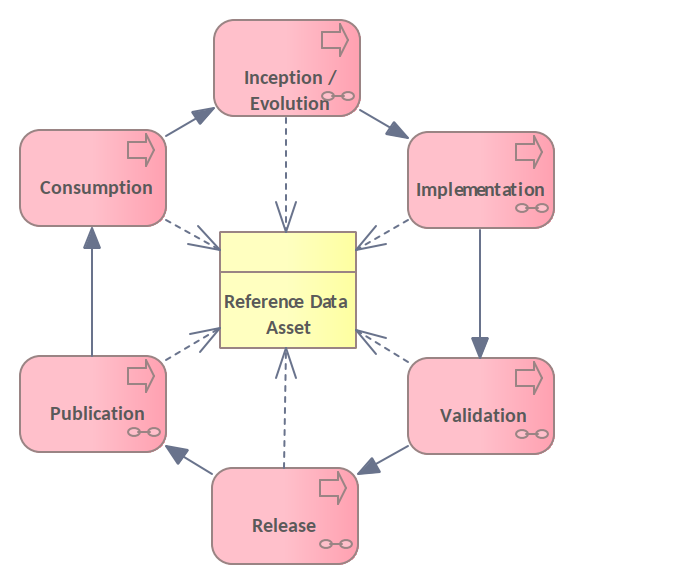
\includegraphics[width=0.6\textwidth]{images/business/Lifecycle process only (new).png}
		\caption{The target architecture of the asset publishing life-cycle}
		\label{fig:lifecycle-new-stages-overview}
	\end{figure}
	
	A more detailed representation of the process life-cycle is provided in Figure \ref{fig:lifecycle-new-overview} below. It is provided here for introducing the reader to the target architecture. The details surrounding this overview are laid out in the next sections. 
	
	\begin{figure}[h]
		\centering
		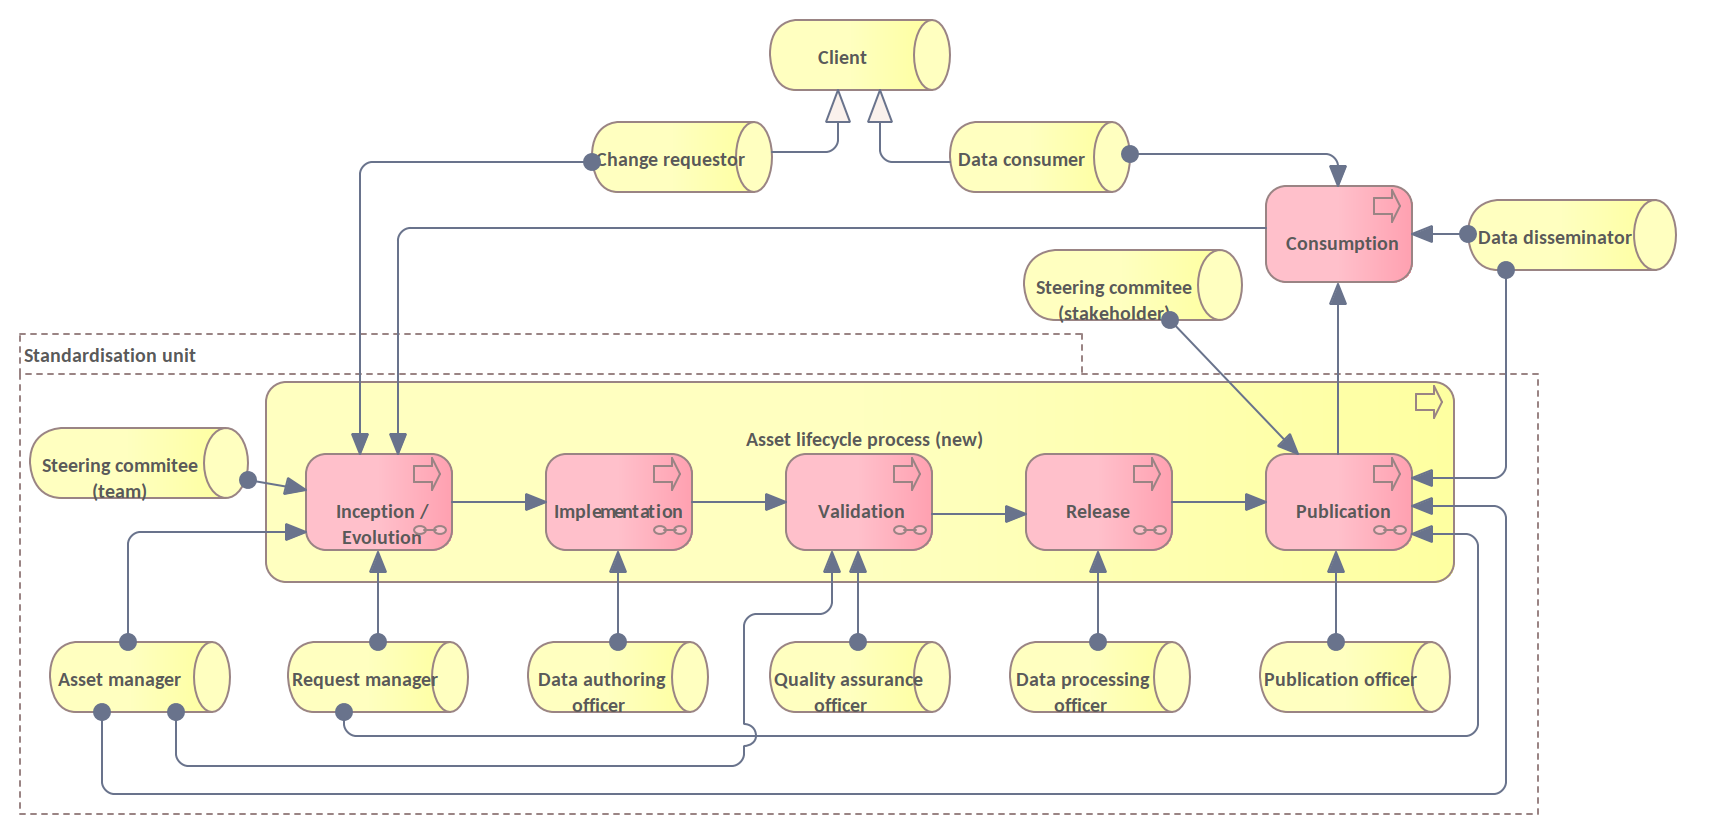
\includegraphics[width=1.05\textwidth]{images/business/Lifecycle (new).png}
		\caption{The new asset life-cycle stages and roles}
		\label{fig:lifecycle-new-overview}
	\end{figure}
	
	The life-cycle process stages, represented by red rectangles with an arrow symbol inside, are linearly sequenced inside the asset lifecycle process, which is placed inside the ``standardisation unit'' box signifying that these processes are executed by the SU, while the ``Consumption'' stage is placed outside meaning that it is an external process and is not in scope. The detailed description of the life-cycle architecture is provided in Section \ref{sec:lifecycle-new}.
	
	The yellow boxes, resembling a cylinder placed around the perimeter of the asset lifecycle, represent agent roles involved in process stages. The arrows indicate in which stage each role participate. As can be seen, one role can participate in multiple stages an required. The derailed definition of roles is provided in Section \ref{sec:lifecycle-roles} and how they are involved is described in Section \ref{sec:lifecycle-new}. Additional details are specified in the business use case scenarios covered in Section \ref{sec:business-use cases} while a contrast to the workflows can be established through Section\ref{sec:lifecycle-current-stages}.